\section{Open interdisciplinary questions}
\label{sec:agenda}

\begin{figure}[t]
  \centering
  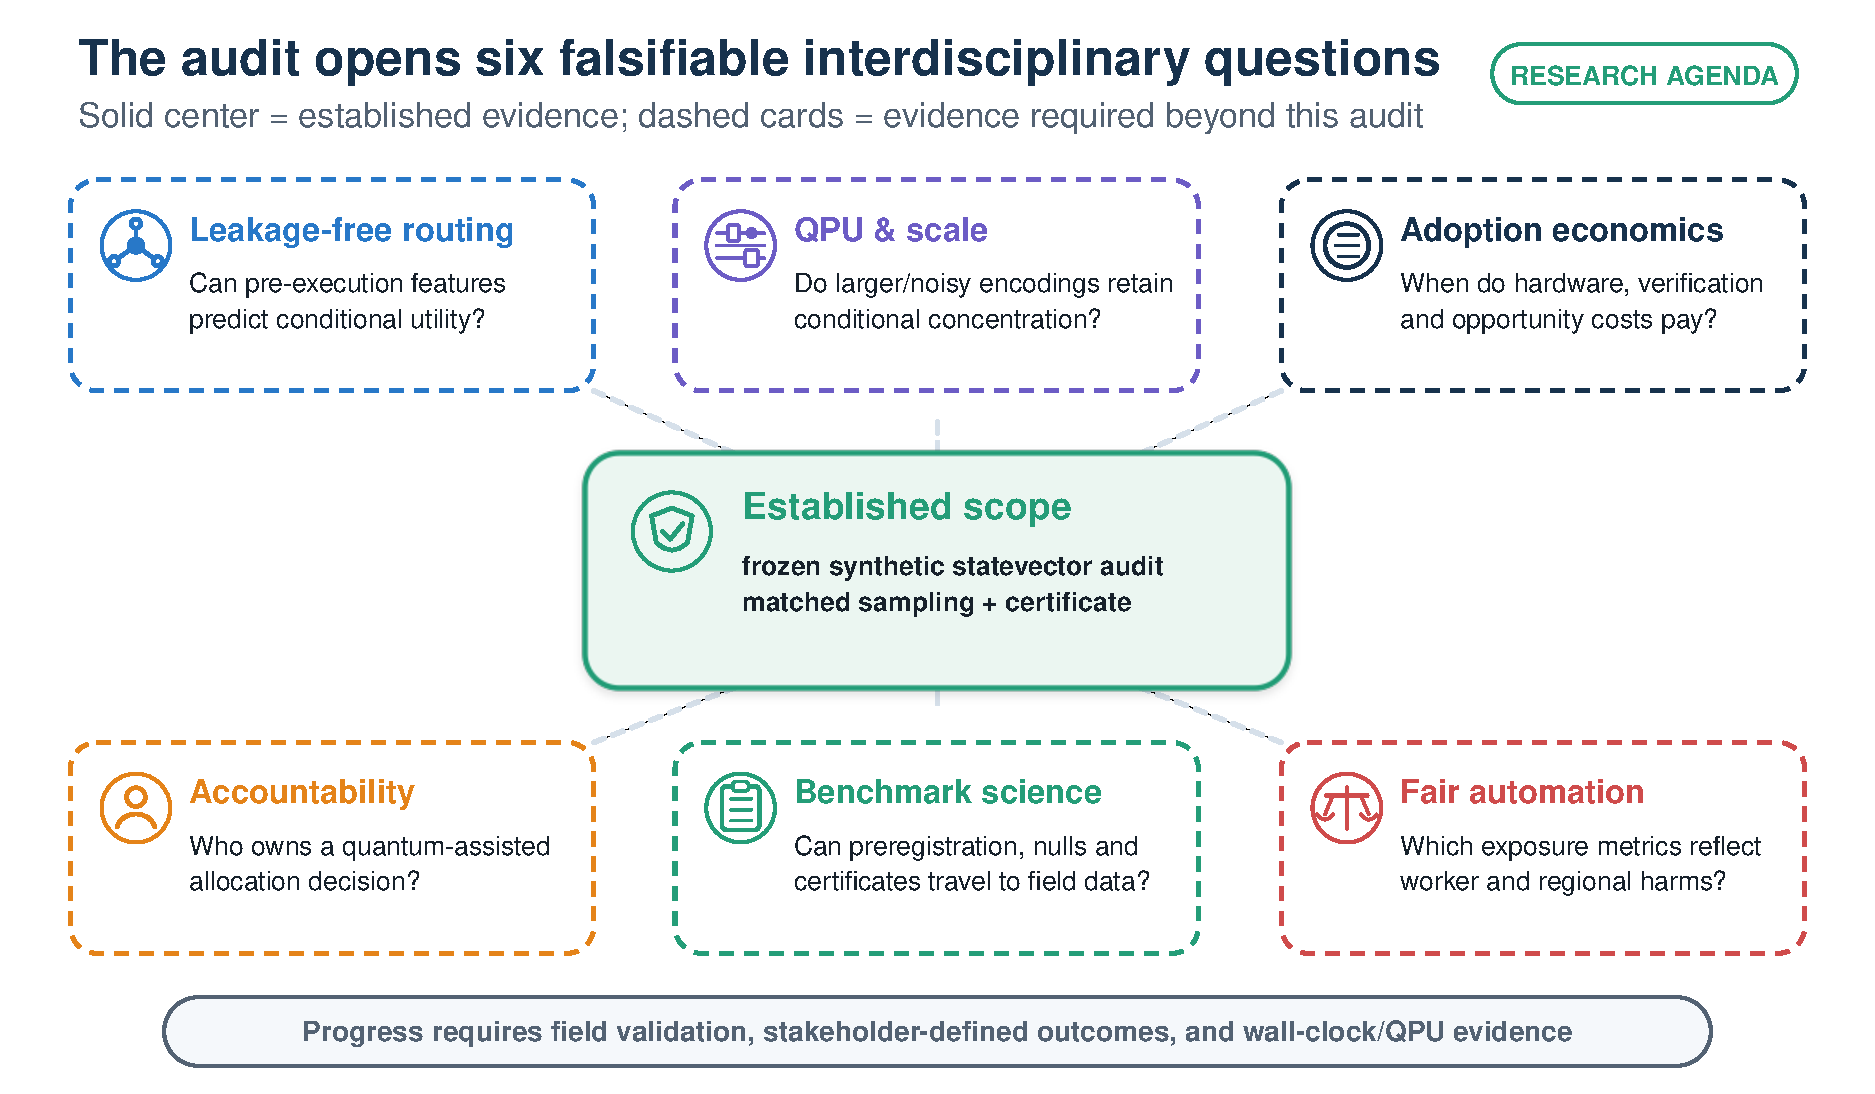
\includegraphics[width=\linewidth]{figs/fig6_open_questions_map.pdf}
  \caption{Research agenda induced by the evidence boundary. The solid center is established here; dashed cards require new field, governance, economic, or quantum-hardware evidence.}
  \label{fig:agenda}
\end{figure}


The evidence boundary exposes six research programs. \textbf{(1) Leakage-free routing:} can pre-execution instance features predict incremental quantum utility under locked, out-of-sample evaluation, connecting selective prediction and algorithm selection~\citep{geifman2017selective,rice1976algorithm,kotthoff2014algorithm}? \textbf{(2) Adoption economics:} when do QPU access, engineering, verification, delay and opportunity costs justify invocation? This is a bounded-rationality and organizational-contracting problem, not merely an algorithmic ratio~\citep{simon1955behavioral,hart1990property}. \textbf{(3) Accountability:} who owns a classically certified but quantum-influenced allocation, and what evidence should a governance system retain~\citep{nist2023airmf,iso42001}? \textbf{(4) Fair automation:} which stakeholder-defined exposure, workload and labor outcomes should replace our simple dispersion term~\citep{selbst2019fairness,bai2022algorithmic}? \textbf{(5) QPU and scale:} does conditional concentration survive larger encodings, noise, compilation and equal-budget optimizer sweeps~\citep{preskill2018nisq,bharti2022nisq}? \textbf{(6) Benchmark science:} can preregistration, null retention and certificates extend to privacy-preserving field data while maintaining reproducibility~\citep{pineau2021reproducibility}? These are falsifiable next steps; none is answered by the present synthetic statevector experiment.
